% 第 1 章
\section{引言：为什么两百年后，直线仍是诚实数据分析的起点}\label{sec:intro}

\subsection{这篇教程要回答的问题}

每一门机器学习课程、每一本统计教材，都会在头两周讲线性回归；而它们几乎都以同样的方式讲：扔给你一个公式
\[
  \widehat{\bm{\beta}} = (\X^\top \X)^{-1} \X^\top \y,
\]
让你记住，然后赶紧奔向「更激动人心」的模型。

这篇教程反着来：每一步都自己挣出来。读完之后，你应该能从第一性原理回答：

\begin{enumerate}[label=(\arabic*)]
  \item 为什么一维回归的斜率是 $\dfrac{\Cov(x,y)}{\Var(x)}$？它和 Pearson 相关系数到底是什么关系？（第 \ref{sec:onedim} 章）
  \item 为什么一条直线能量出 $x$ 与 $y$ 的\textit{相关性}，却不能告诉你因果的\textit{方向}？（第 \ref{sec:onedim} 章）
  \item 为什么平方误差？换别的损失会丢掉什么？（第 \ref{sec:why-square} 节）
  \item 高维情形下，当样本量 $n$ 远大于维度 $d$ 时，为什么最小二乘有闭式解 $\widehat{\bm{\beta}} = (\X^\top\X)^{-1}\X^\top\y$？这个解何时唯一、何时最优？（第 \ref{sec:highdim} 章）
  \item 当 $n$ 不再远大于 $d$ 时，是什么先坏掉，修复又是什么？（第 \ref{sec:hd-break} 节）
  \item 把闭式解与梯度下降迭代放在一起，$\widehat{\bm{\beta}}_t$ 有怎样的精确解？不动点意味着什么？（第 \ref{sec:gd} 章）
  \item 当 $d > n$、解已成流形时，迭代收敛到哪里？它与伪逆解是什么关系？（第 \ref{sec:gd-underdet} 章）
  \item 回归系数与协方差、精度矩阵是什么关系？「估计」如何升级为「推断」——即 from estimate to inference？（第 \ref{sec:ggm} 章）
  \item 当观测特征其实是潜变量的非线性投影时，线性回归为何表现为一个核方法？（第 \ref{sec:kernel} 章）
\end{enumerate}

\subsection{一个两百岁、拒绝退休的想法}

最小二乘法由 Legendre（1805）首次发表，Gauss（1809）独立提出并从概率论角度给出了完整推导——后者用它从有噪声的天文观测中预测了谷神星（Ceres）的轨道\cite{legendre1805,gauss1809}。这个方法熬过了此后每一次范式更替：计算机、自助法（bootstrap）、深度学习革命。原因只有一个：

\begin{keybox}[本教程的论点]
线性回归流行，不是因为现实世界是线性的——它很少是。它流行是因为：
\begin{enumerate}[label=(\roman*)]
  \item 局部线性近似常常足够好（Taylor 定理保证了任何光滑函数在局部都是近线性的）；
  \item 它是\textit{唯一可精确求解、可解释、可审计}的基线——其余一切模型都是对照它来衡量自己的；
  \item 它是 logistic 回归、广义线性模型、核方法乃至神经网络输出层的地基。
\end{enumerate}
\end{keybox}

\begin{figure}[htbp]
  \centering
  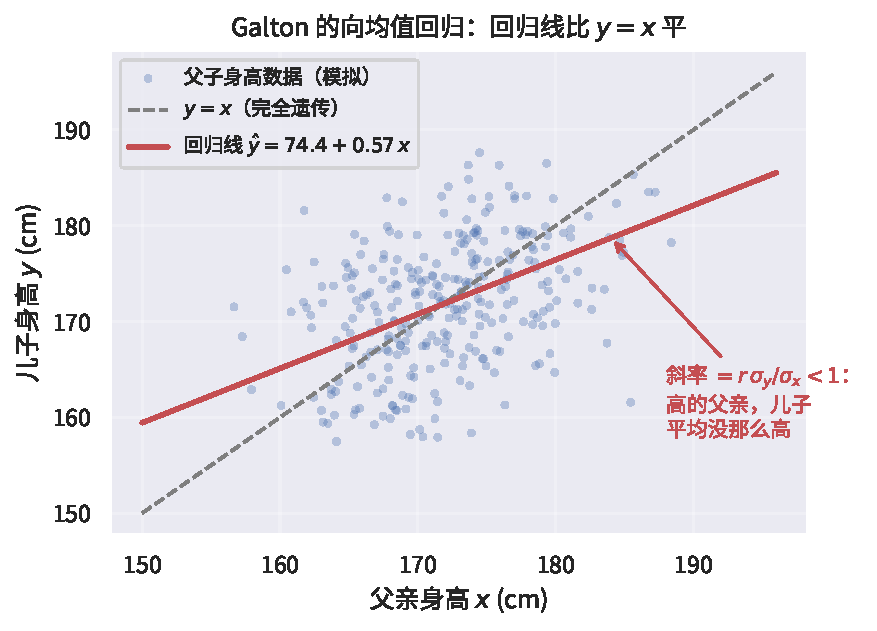
\includegraphics[width=0.8\linewidth]{figures/ch1_galton.pdf}
  \caption{Galton 的「向均值回归」（模拟数据重现）：回归线（红）始终比 $y=x$（灰虚线）平——斜率 $=r\,\sigma_y/\sigma_x$，只要 $|r|<1$，极端必然后退。两百年后，这条直线仍是数据分析的默认起点。}
  \label{fig:ch1-galton}
\end{figure}

\subsection{预备知识}

\begin{itemize}
  \item \textbf{微积分}：偏导数、链式法则，以及「光滑函数的极值出现在导数为零处」这一事实；
  \item \textbf{线性代数}：向量、矩阵、矩阵乘法、转置、逆；「矩阵乘向量是列的线性组合」这一读法；
  \item \textbf{概率}（第 2 章用到）：期望、方差、协方差、相关系数。
\end{itemize}

其余皆在文中推导。

\subsection{记号，只说一次}

一维情形：$n$ 对观测 $(x_i, y_i) \in \R^2$，$i = 1, \dots, n$。高维情形：响应 $y_i \in \R$，特征 $\x_i = (x_{i1}, \dots, x_{id})^\top \in \R^d$，设计矩阵 $\X \in \R^{n \times d}$（行为 $\x_i^\top$），参数 $\bbeta \in \R^d$。误差项 $\varepsilon_i$ 收纳一切直线解释不了的东西：测量噪声、遗漏的变量、真实的随机性，以及「用超平面近似非线性世界」这一罪过本身。

约定：
\[
  \bar{x} = \frac{1}{n}\sum_{i=1}^n x_i, \qquad
  \Var_n(x) = \frac{1}{n}\sum_{i=1}^n (x_i - \bar{x})^2, \qquad
  \Cov_n(x, y) = \frac{1}{n}\sum_{i=1}^n (x_i - \bar{x})(y_i - \bar{y}),
\]
即以 $n$ 为分母的样本方差与协方差（用 $n-1$ 只会给比值带来一个无关紧要的因子）。全程用 $\Var$、$\Cov$ 表示对随机变量取期望的总体量，用下标 $n$ 表示样本量。
